

%\documentclass{book}\begin{document}<content\end{document}
\documentclass[letter, 11pt, margins=0.3in]{texMemo}  % The texMemo package by Rob Oakes.

\usepackage{amsmath}
\usepackage{color, soul}
\usepackage{dcolumn}
\usepackage{enumitem}

    \newcolumntype{d}[1]{D{.}{.}{#1}}
\usepackage[colorlinks=true, citecolor=blue]{hyperref}

\usepackage{graphicx, lipsum}

\usepackage{imakeidx}

\usepackage{caption}
\usepackage{subcaption}

\usepackage[LGRgreek]{mathastext}

\usepackage{listings}
\usepackage[]{matlab-prettifier}

\usepackage{multirow}

\usepackage{natbib}
\bibliographystyle{apalike}

\usepackage{printlen}  % \printlength\textwidth - To determine textwidth of document.  Here is it 496 pt.

\usepackage{siunitx}

\usepackage{tablefootnote}

\usepackage[table]{xcolor}
\definecolor{maroon}{cmyk}{0,0.87,0.68,0.32}
\definecolor{LightCyan}{rgb}{0.88,1,1}
\definecolor{Gray}{gray}{0.85}


\newcommand{\is}[1]{%
\if@noftnote%
\index{#1}%
\else%
\index{#1|fn{\number\value{footnote}}}%
\fi%
}

\makeindex


\graphicspath{ {../} }


\memodate{\today~(Submitted)}
\memosubject{ACS 547, Noise Control Applications - Module 2 Assignment\\}



\begin{document}

\maketitle


\vspace{-0.25cm}
\section*{Problem 1 - Washing Machine Mount Design (1 DOF)}


\subsection*{Problem 1a}

The Matlab code for this problem is listed in Appendix~\ref{appendix:problem1}.

\vspace{0.25cm}
Figure~\ref{figure:1aLoadForceVersusRPM} shows the load force produced by the 1 kg imbalanced mass at a 0.5 m radius from the center of the washing machine as a function of angular speed in RPM.

\vspace{-0.25cm}
\begin{figure}[htb!]
    \center
        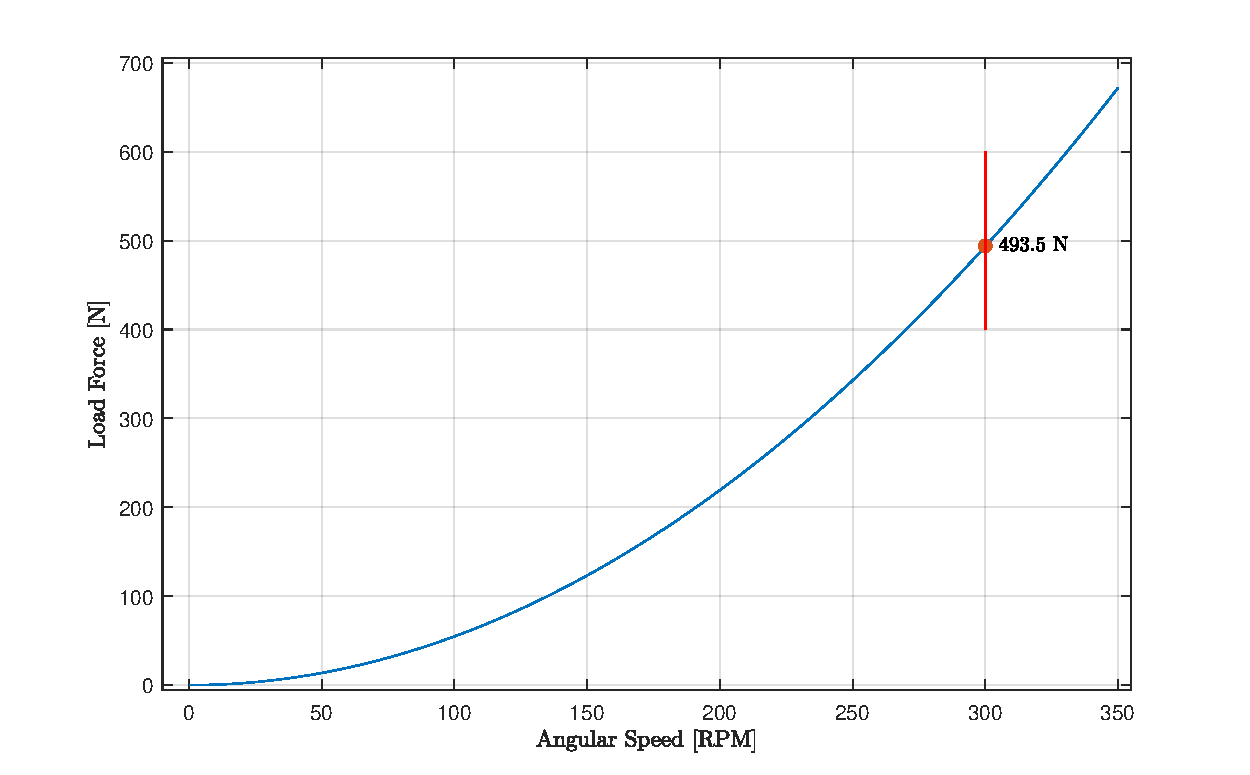
\includegraphics[scale = 0.7, keepaspectratio]{Homework_3_Part_1a.pdf}
    \caption{Load force of 1 kg imbalanced mass at a 0.5 m radius versus washing machine angular speed.}
    \label{figure:1aLoadForceVersusRPM}
\end{figure}

\vspace{0.25cm}
The force amplitude is 493.5 N at a frequency of 5 Hz when the washing machine operates at 300 RPM.





\subsection*{Problem 1b}

The static displacement of the load in the washing machine must be less than 1 cm (i.e., the deflection is calculated with only the 10 kg load mass).  The corresponding mount stiffness, $k_s$, is \textbf{9,810 $\frac{N}{m}$}.

\vspace{0.25cm}
The natural frequency, $w_o$, of the mount is \textbf{1.5 Hz} (or 9.4 $\frac{radians}{s}$).




\newpage
\subsection*{Problem 1c}

Figure~\ref{figure:1cTransmissionLoss} shows the transmission loss of the system for a set of damping ratios ranging from 0.001 to 1.

\vspace{-0.25cm}
\begin{figure}[htb!]
    \center
        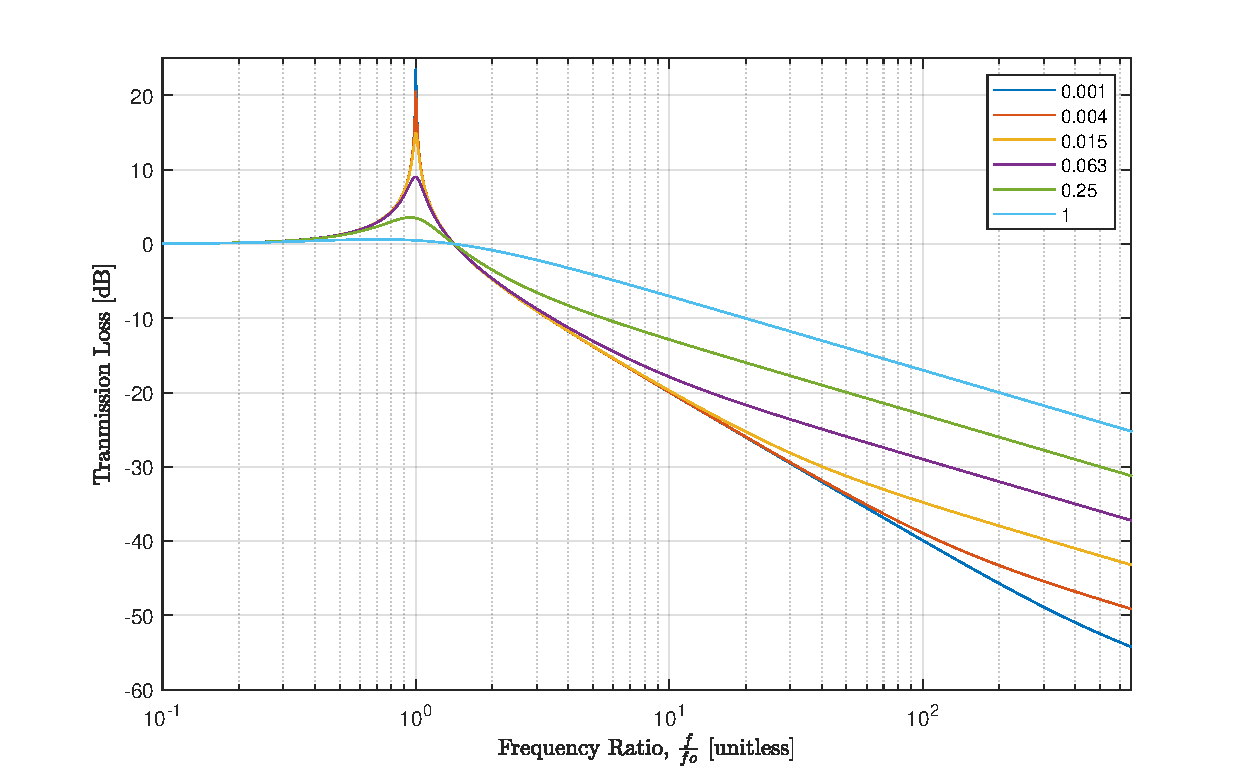
\includegraphics[scale = 0.7, keepaspectratio]{Homework_3_Part_1c.pdf}
    \caption{Transmission loss of the system.  Its natural frequency is 1.5 Hz.}
    \label{figure:1cTransmissionLoss}
\end{figure}





\subsection*{Problem 1d}

Figure~\ref{figure:1dAppliedForce} shows the force applied to the foundation as a function of RPM.

\vspace{-0.25cm}
\begin{figure}[htb!]
    \center
        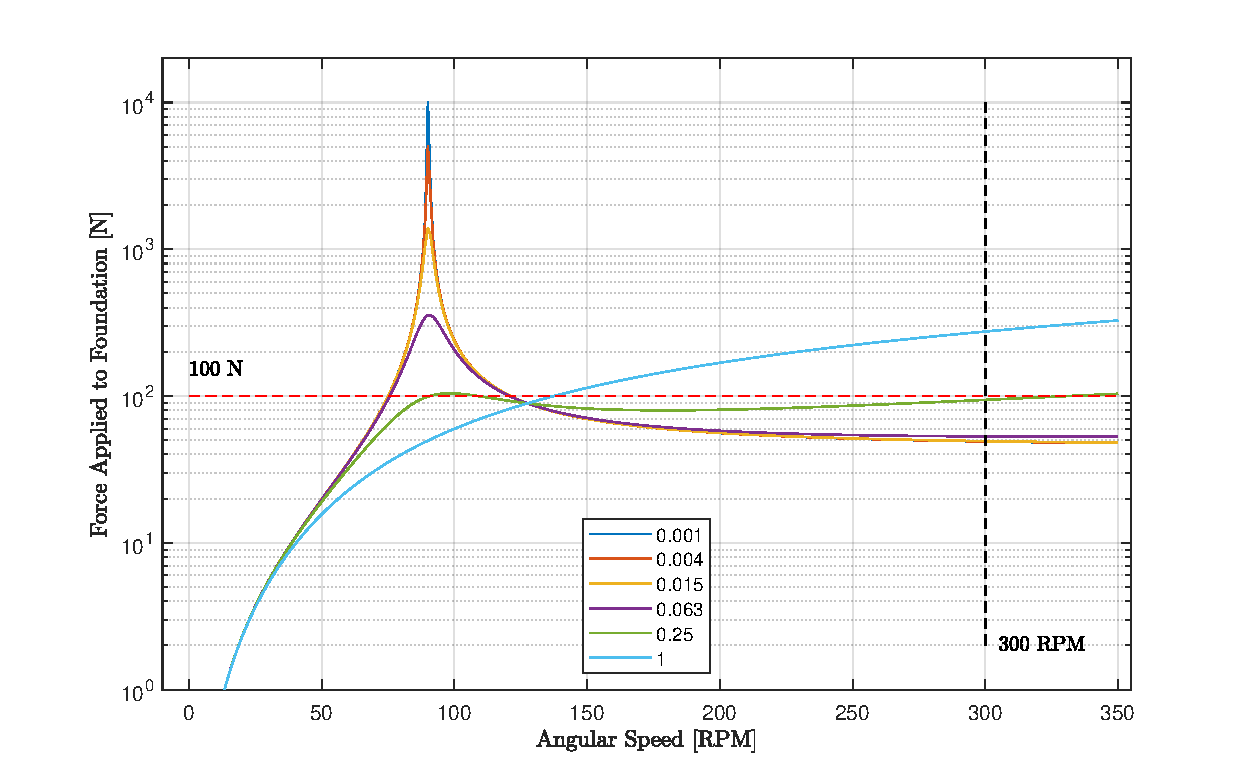
\includegraphics[scale = 0.7, keepaspectratio]{Homework_3_Part_1d.pdf}
    \caption{Force applied to the foundation versus RPM.}
    \label{figure:1dAppliedForce}
\end{figure}

There is no damping ratio for which the applied force is less than 100 N across the whole operating range.  The best damping ratio is $\zeta = 0.25$.  With this damping ratio, the force applied to the foundation still exceeds the 100 N target in two regions:  91 to 109 RPM and 331 to 350 RPM.  In both regions the force is about 104 N.





\subsection*{Problem 1e}

Figure~\ref{figure:1eAdmittance} shows the admittance as a function of RPM.

\vspace{-0.25cm}
\begin{figure}[htb!]
    \center
        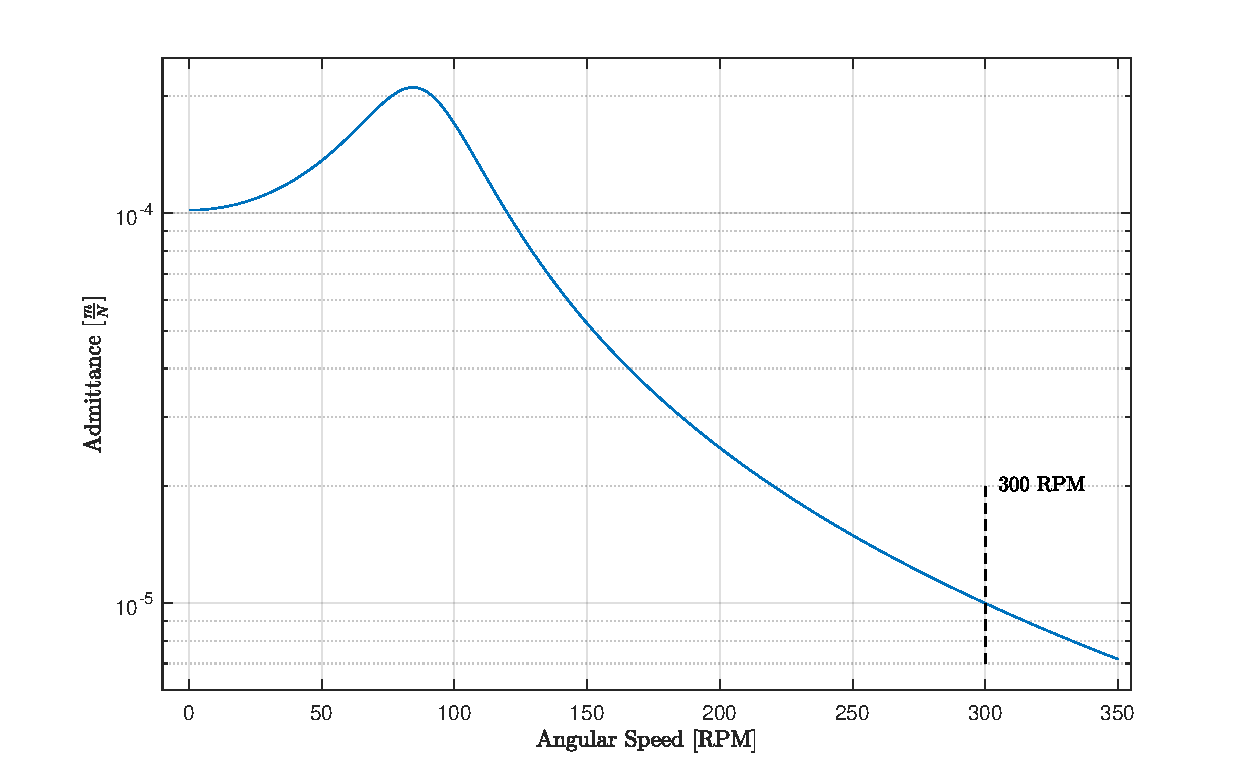
\includegraphics[scale = 0.7, keepaspectratio]{Homework_3_Part_1e.pdf}
    \caption{Admittance versus RPM.}
    \label{figure:1eAdmittance}
\end{figure}

The admittance at 300 RPM is 1e-5 $\frac{m}{N}$.





\subsection*{Problem 1f}

Figure~\ref{figure:1fDisplacement} shows the displacement of the washing machine as a function of RPM.

\vspace{-0.25cm}
\begin{figure}[htb!]
    \center
        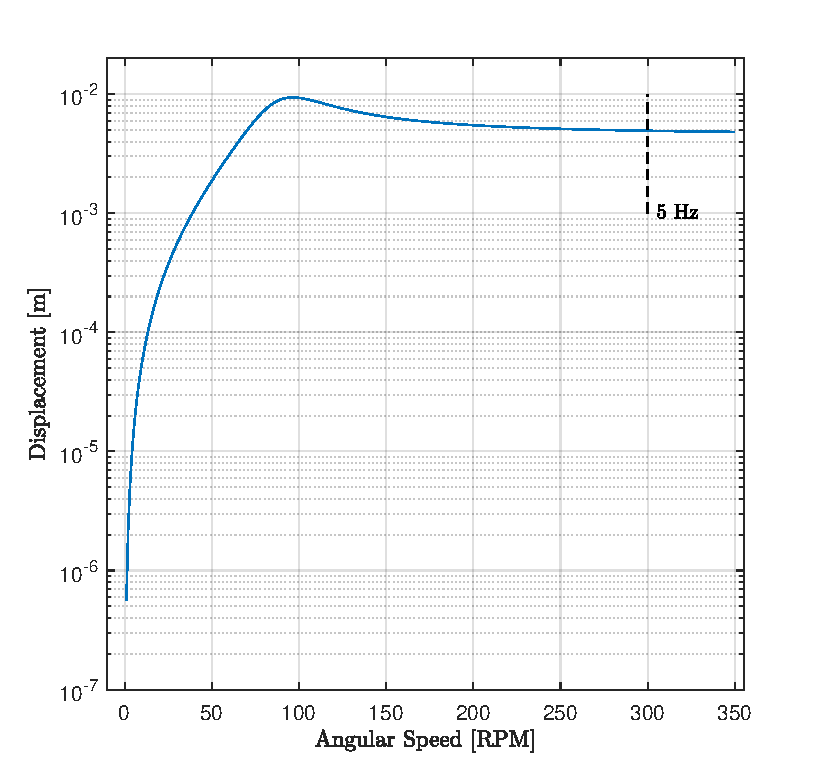
\includegraphics[scale = 0.7, keepaspectratio]{Homework_3_Part_1f.pdf}
    \vspace{-0.2cm}
    \caption{Displacement versus RPM.}
    \label{figure:1fDisplacement}
\end{figure}

The displacement of the washing machine at 300 RPM is \SI{5e-3}~~$m$.  This amount of displacement for the 300 RPM operating state seems excessive.  The washing machine undergoes larger momentary displacements as is spins up to the 300 RPM operating state, in particular around 100 RPM.









\newpage
\section*{Problem 2 - Washing Machine Mount Design (2 DOF)}
\setcounter{figure}{0}


\subsection*{Problem 2a}

The Matlab code for this problem is listed in Appendix~\ref{appendix:problem2}.

\vspace{0.25cm}
Figure~\ref{figure:2aDiagramTwoStageMount} illustrates the two-stage vibration mount considered here (see slide 8 of 42 for Lecture 14 on Monday, March 3, 2025).  Modeling will be done using discrete viscous damping elements.

\vspace{-0.25cm}
\begin{figure}[htb!]
    \center
        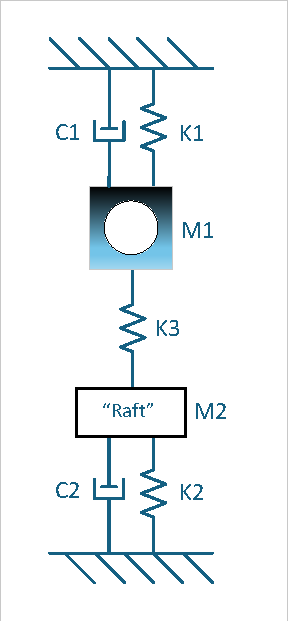
\includegraphics[scale = 0.7, keepaspectratio, trim=4 4 4 4, clip]{ACS 547 - Homework 3, Problem 2.pdf}
    \vspace{-0.2cm}
    \caption{Two-stage vibration mount system for the washing machine.}
    \label{figure:2aDiagramTwoStageMount}
\end{figure}



\newpage
\subsection*{Problem 2b}

Table~\ref{table:2Parameters} lists the initial stiffness and damping coefficients for the system.

\vspace{0.25cm}
\setlength{\abovecaptionskip}{1.5pt}
\vspace{0.1cm}
{\renewcommand{\arraystretch}{1.5}
\begin{table}[htpb!]

    \footnotesize

    \centering

        \begin{tabular}{ | c | c | c | }
        \hline
        \textbf{M1}  &  110  &  $kg$   \\
        \hline
        \textbf{K1}  &  100  &  $\frac{N}{m}$  \\
        \hline
        \textbf{C1}  &  5  &  $\frac{kg}{s}$  \\
        \hline
        \end{tabular}
        \hfill
        \begin{tabular}{ | c | c | c | }
        \hline
        \textbf{M2}  &  100  &  $kg$   \\
        \hline
        \textbf{K2}  &  100  &  $\frac{N}{m}$  \\
        \hline
        \textbf{C2}  &  5  &  $\frac{kg}{s}$  \\
        \hline
        \end{tabular}
        \hfill
        \begin{tabular}{ | c | c | c | }
        \hline
        \textbf{M3}  &  0  &  $kg$   \\
        \hline
        \textbf{K3}  &  1,000  &  $\frac{N}{m}$  \\
        \hline
        \textbf{C3}  &  5  &  $\frac{kg}{s}$  \\
        \hline
        \end{tabular}

        \vspace{0.5cm}
        \caption{Initial values of stiffness and damping coefficients.}
        \label{table:2Parameters}

\end{table}



\subsection*{Problem 2c}

\vspace{0.25cm}
Figure~\ref{figure:2cAdmittance} illustrates the admittance of the washing machine and the raft with the force applied to the washing machine.

\vspace{0.25cm}
At the operating speed of 300 RPM, the admittance of the washing machine is \SI{9.31e-6}~~$\frac{m}{N}$.

\vspace{-0.25cm}
\begin{figure}[htpb!]
    \center
        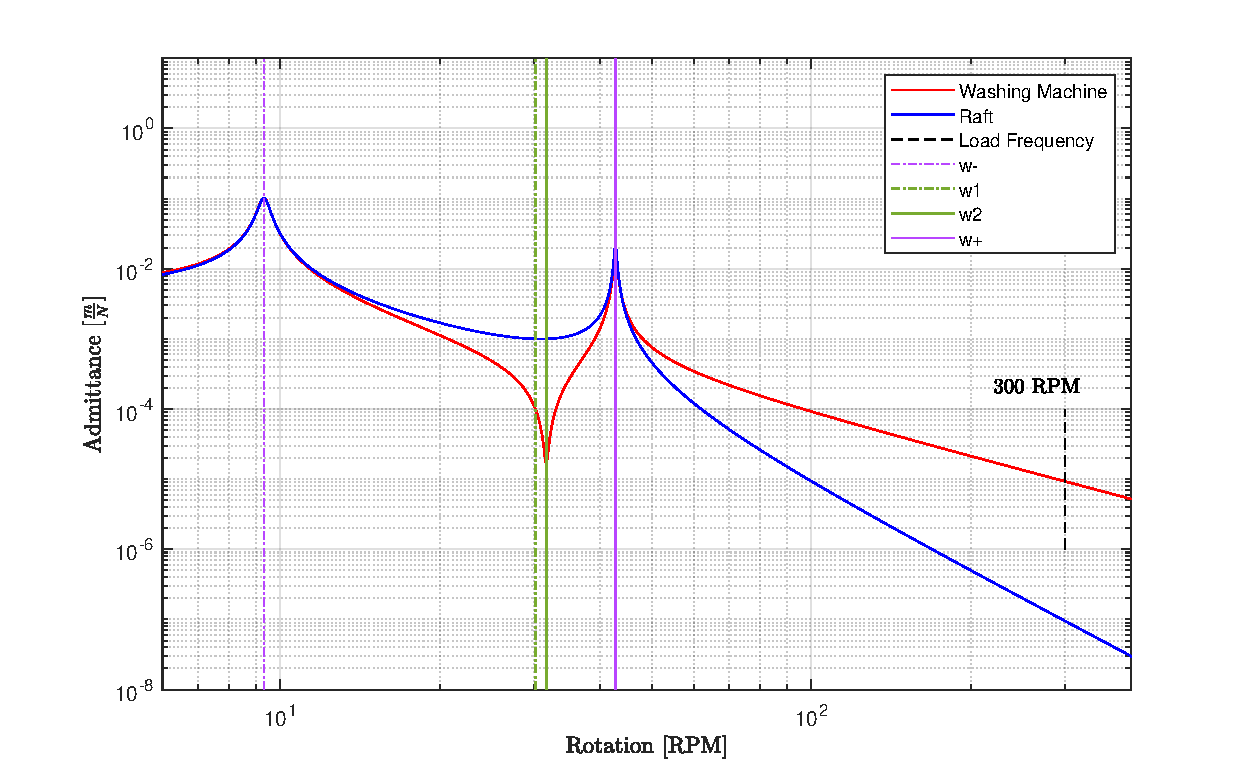
\includegraphics[scale = 0.7, keepaspectratio, trim=4 4 4 4, clip]{Homework_3_Part_2c.pdf}
    \vspace{0.25cm}
    \caption{Admittance of the washing machine and the raft with a force on the washing machine.}
    \label{figure:2cAdmittance}
\end{figure}



\subsection*{Problem 2d}

\vspace{0.25cm}
Figure~\ref{figure:2dDisplacement} illustrates the displacement of the washing machine and the raft with the force applied to the washing machine.

\vspace{-0.25cm}
\begin{figure}[htpb!]
    \center
        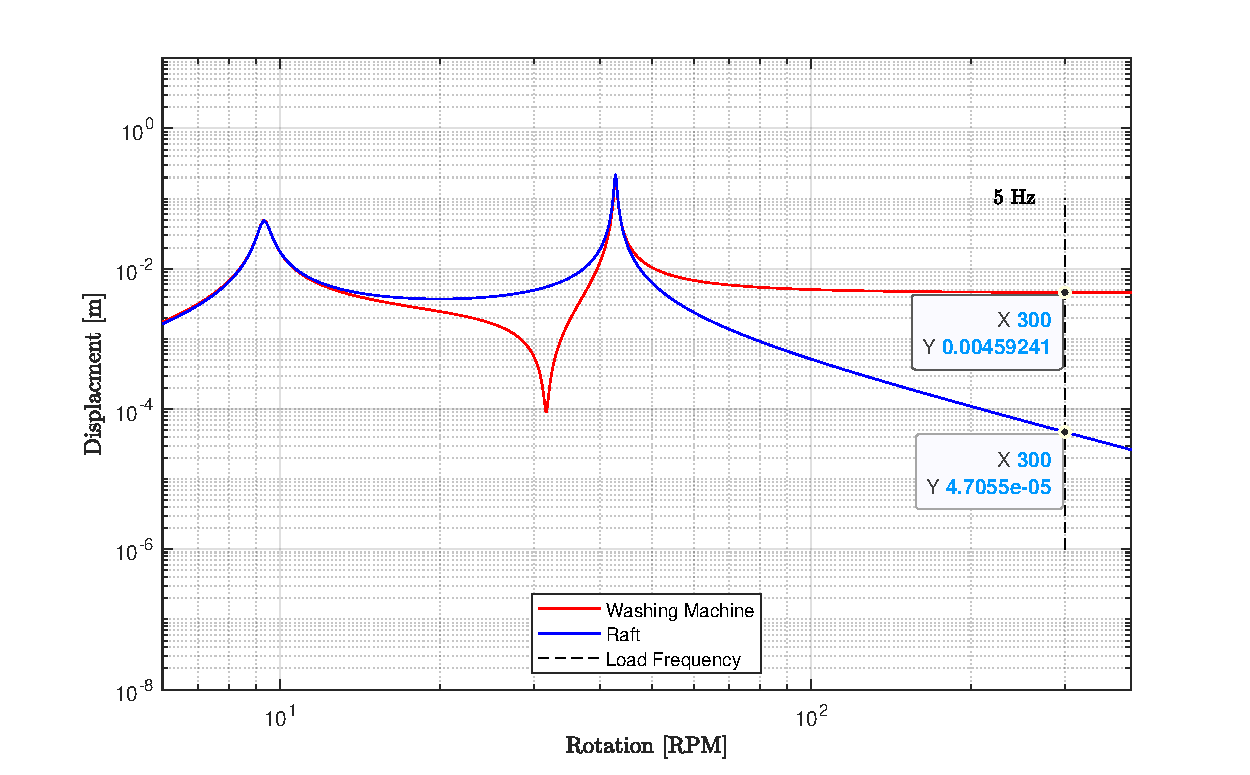
\includegraphics[scale = 0.7, keepaspectratio, trim=4 4 4 4, clip]{Homework_3_Part_2d.pdf}
    \vspace{0.25cm}
    \caption{Displacement of the washing machine and the raft with a force on the washing machine.}
    \label{figure:2dDisplacement}
\end{figure}

\vspace{0.25cm}
At the operating speed of 300 RPM, the displacement of the washing machine is \SI{4.6e-3}~~$m$, which is less than the \SI{5.0e-3}~~$m$ displacement with the first-order system.

The displacement of the raft is \SI{4.7e-5}~~$m$.



\subsection*{Problem 2e}

\vspace{0.25cm}
Figure~\ref{figure:2eLoadForce} illustrates the force applied to the ground by the raft.  This is calculated by multiplying the displacement of the raft by the K2 spring constant.

The load on the ground is always less than 100 $N$.

\vspace{-0.25cm}
\begin{figure}[htpb!]
    \center
        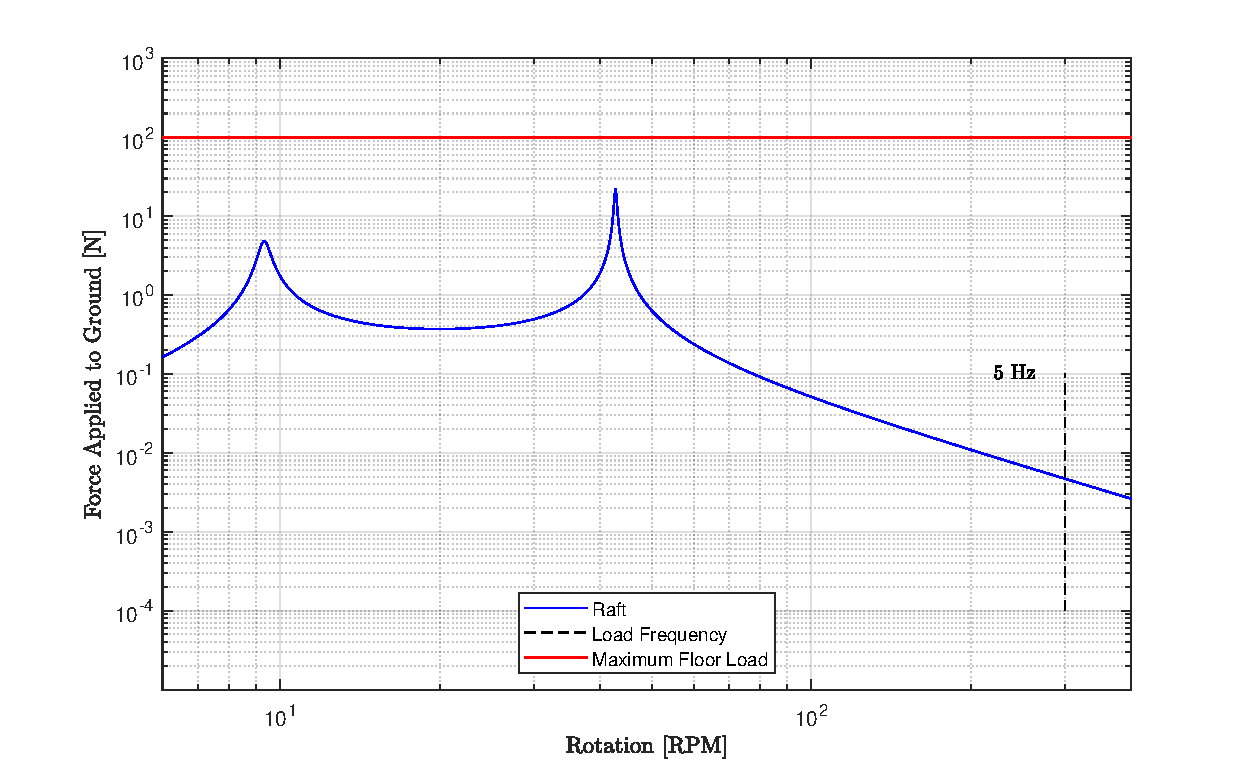
\includegraphics[scale = 0.7, keepaspectratio, trim=4 4 4 4, clip]{Homework_3_Part_2e.pdf}
    \vspace{0.25cm}
    \caption{Force applied to the ground by the raft.}
    \label{figure:2eLoadForce}
\end{figure}



\subsection*{Problem 2f}

\vspace{0.25cm}
The initial parameter set chosen, see Table~\ref{table:2bParameters}, facilitated a displacement of the washing machine of \SI{4.6e-3}~~$m$ at 300 RPM, which is less than the \SI{5.0e-3}~~$m$ found for the 1 DOF system.  The force applied to the ground by the raft is less than the required 100 $N$ maximum.



\subsection*{Problem 2g}

\vspace{0.25cm}
The initial parameter set chosen, see Table~\ref{table:2bParameters}, facilitated a displacement of the washing machine of \SI{4.6e-3}~~$m$ at 300 RPM, which is less than the \SI{5.0e-3}~~$m$ found for the 1 DOF system.  The force applied to the ground by the raft is less than the required 100 $N$ maximum.







\newpage
\section*{Problem 3 - Washing Machine Dynamic Vibration Absorber Design}
\setcounter{figure}{0}


The Matlab code for this problem is listed in Appendix~\ref{appendix:problem3}.


\subsection*{Part 3a}

Figure~\ref{figure:3aDiagramDVA} illustrates the dynamic vibration absorber (DVA) system.

\vspace{-0.25cm}
\begin{figure}[htb!]
    \center
        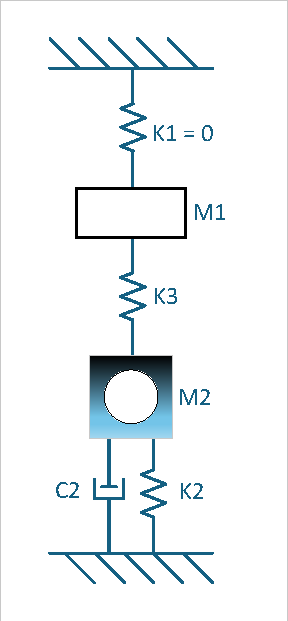
\includegraphics[scale = 0.7, keepaspectratio, trim=4 4 4 4, clip]{ACS 547 - Homework 3, Problem 3 DVA.pdf}
    \caption{Dynamic vibration absorber system for the washing machine.}
    \label{figure:3aDiagramDVA}
\end{figure}

Table~\ref{table:3Parameters} lists the stiffness and damping coefficients for the system.

\vspace{0.25cm}
\setlength{\abovecaptionskip}{1.5pt}
\vspace{0.1cm}
{\renewcommand{\arraystretch}{1.5}
\begin{table}[htpb!]

    \footnotesize

    \centering

        \begin{tabular}{ | c | c | c | }
        \hline
        \textbf{M1}  &  15  &  $kg$   \\
        \hline
        \textbf{K1}  &  0  &  $\frac{N}{m}$  \\
        \hline
        \textbf{C1}  &  0  &  $\frac{kg}{s}$  \\
        \hline
        \end{tabular}
        \hfill
        \begin{tabular}{ | c | c | c | }
        \hline
        \textbf{M2}  &  110  &  $kg$   \\
        \hline
        \textbf{K2}  &  9,810  &  $\frac{N}{m}$  \\
        \hline
        \textbf{C2}  &  1,962  &  $\frac{kg}{s}$\tablefootnote{0.2 fraction of respective spring stiffness.}  \\
        \hline
        \end{tabular}
        \hfill
        \begin{tabular}{ | c | c | c | }
        \hline
        \textbf{M3}  &  0  &  $kg$   \\
        \hline
        \textbf{K3}  &  1e5  &  $\frac{N}{m}$  \\
        \hline
        \textbf{C3}  &  1e4  &  $\frac{kg}{s}$\tablefootnote{0.1 fraction of respective spring stiffness.}  \\
        \hline
        \end{tabular}

        \vspace{0.5cm}
        \caption{Stiffness and damping coefficients for the DVA system.}
        \label{table:3Parameters}

\end{table}


Damping was implemented by adding with an imaginary component to the respective spring stiffness\footnote{Not equivalent to using a damping vector in the argument to the given Matlab nDOF function script-file.}.



\newpage
\subsection*{Part 3b}

Figure~\ref{figure:3aEquationsFromDvaLecture} shows the admittance response of the original system and DVA system based on the equations presented in the tutorial lecture on DVA system analysis.

\vspace{-0.25cm}
\begin{figure}[htpb!]
    \center
        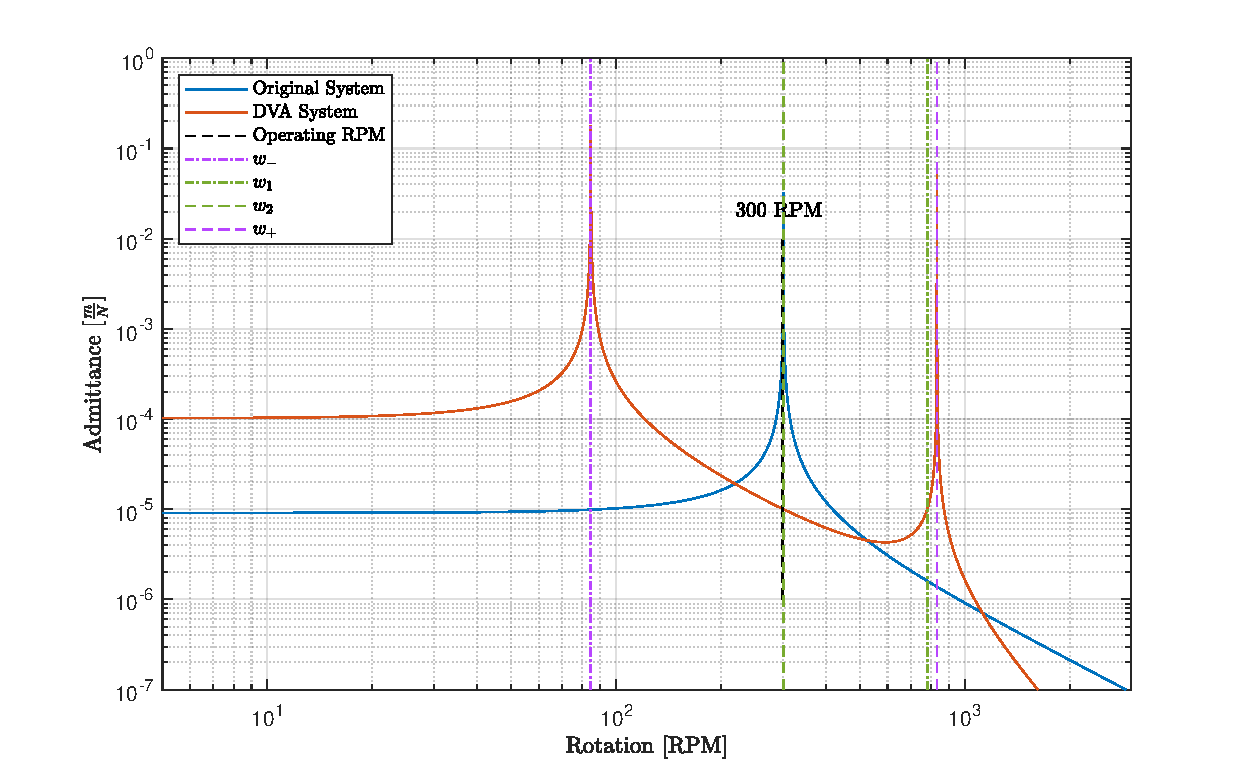
\includegraphics[scale = 0.7, keepaspectratio, trim=4 4 4 4, clip]{Homework_3_Part_3a.pdf}
    \caption{Admittance responses based on the equations from the DVA tutorial lecture.}
    \label{figure:3aEquationsFromDvaLecture}
\end{figure}



\subsection*{Part 3c}

Figure~\ref{figure:3bAdmittance} shows the admittance response of the DVA system using the nDOF function script-file.  The stiffness of the coupling spring, $k_3$, is set to place the null of the admittance response at the 300 RPM operating state of the washing machine.

\vspace{-0.25cm}
\begin{figure}[htpb!]
    \center
        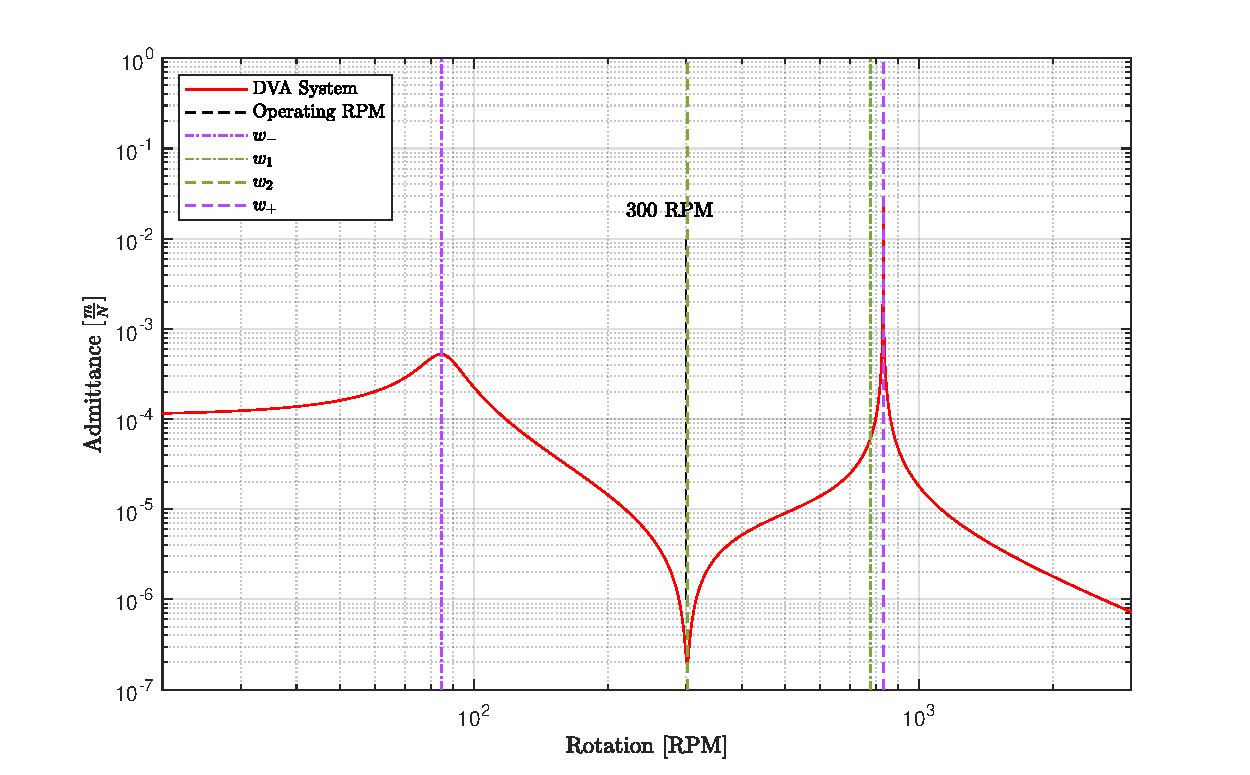
\includegraphics[scale = 0.7, keepaspectratio, trim=4 4 4 4, clip]{Homework_3_Part_3b.pdf}
    \caption{Solution using nDOF script-file function.}
    \label{figure:3bAdmittance}
\end{figure}

Added damping to the DVA system reduces the prominence of its two resonant peaks.



\subsection*{Part 3d}

\vspace{0.25cm}
Figure~\ref{figure:3cDisplacement} ph

The ramp up to 300 RPM occurs quickly so that the large displacements are transient.

\vspace{-0.25cm}
\begin{figure}[htpb!]
    \center
        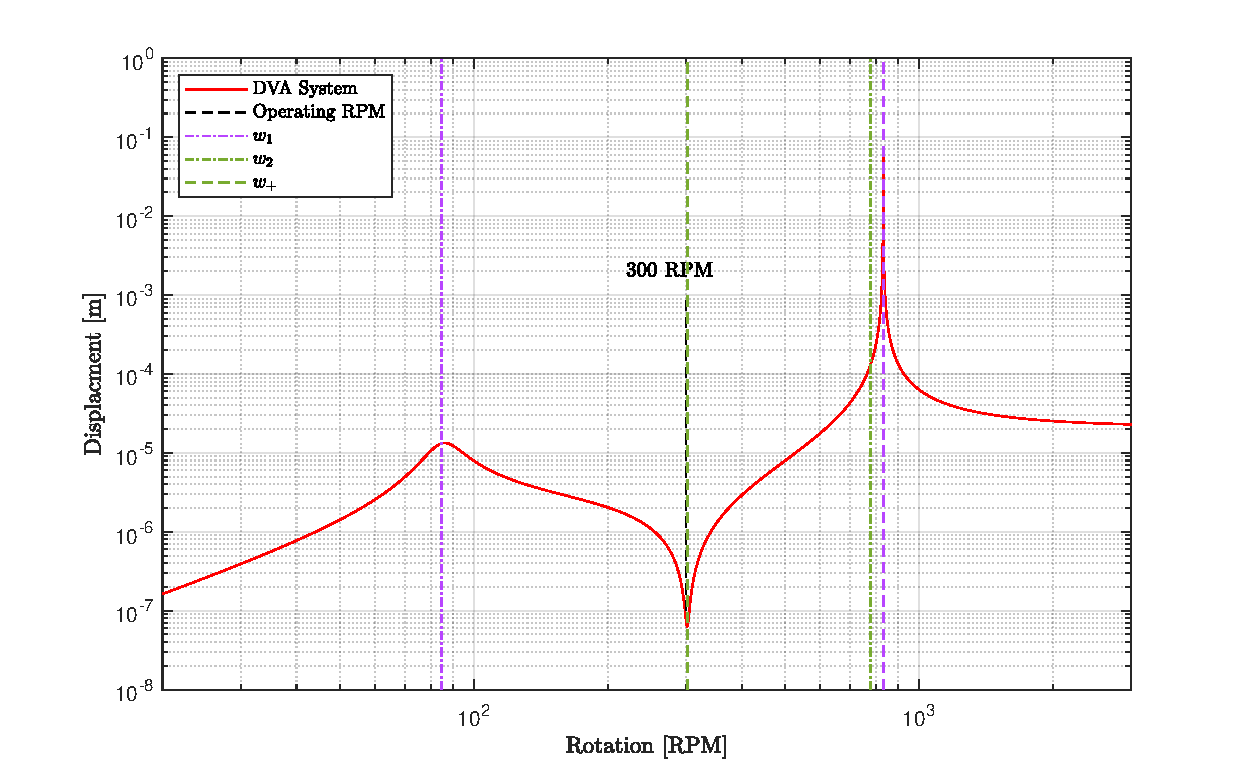
\includegraphics[scale = 0.7, keepaspectratio, trim=4 4 4 4, clip]{Homework_3_Part_3c.pdf}
    \vspace{0.25cm}
    \caption{Displacement of the washing machine.}
    \label{figure:3cDisplacement}
\end{figure}



\subsection*{Part 3e}

\vspace{0.25cm}
Figure~\ref{figure:3dForce} ph

ph

\vspace{-0.25cm}
\begin{figure}[htpb!]
    \center
        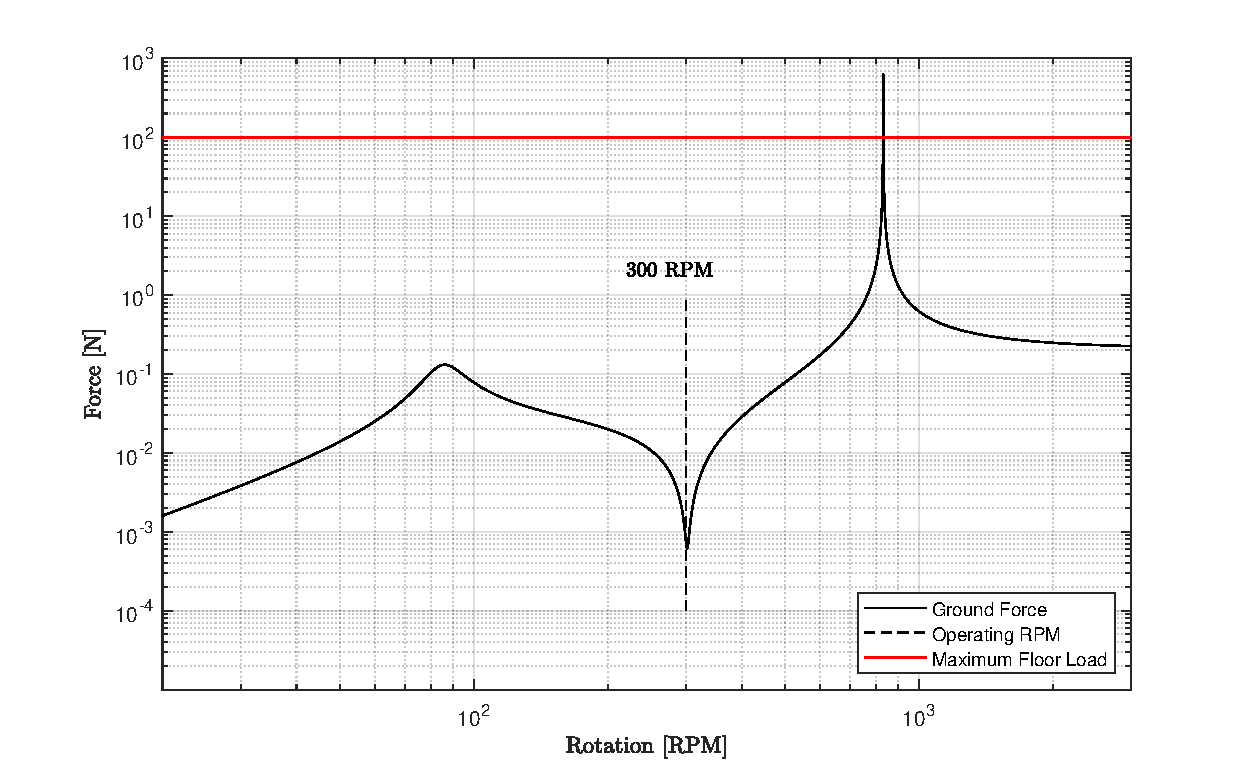
\includegraphics[scale = 0.7, keepaspectratio, trim=4 4 4 4, clip]{Homework_3_Part_3d.pdf}
    \vspace{0.25cm}
    \caption{Force applied to the floor.}
    \label{figure:3dForce}
\end{figure}







\newpage
\section*{Problem 4 - Washing Machine Abuse Testing}
\setcounter{figure}{0}


The Matlab code for this problem is listed in Appendix~\ref{appendix:problem4}.


\subsection*{Part 3a}










\newpage
\section{Appendix - Matlab Code for Problem 1}
\label{appendix:problem1}

\lstinputlisting[style=Matlab-editor, numbers=left, mlshowsectionrules, basicstyle=\scriptsize]{../ACS_547_Module_3_Question_1_Monday_March_3_2025.m}


\newpage
\section{Appendix - Matlab Code for Problem 2}
\label{appendix:problem2}

\lstinputlisting[style=Matlab-editor, numbers=left, mlshowsectionrules, basicstyle=\scriptsize]{../ACS_547_Module_3_Question_2_Monday_March_3_2025.m}


\newpage
\section{Appendix - Matlab Code for Problem 3}
\label{appendix:problem3}

\lstinputlisting[style=Matlab-editor, numbers=left, mlshowsectionrules, basicstyle=\scriptsize]{../ACS_547_Module_3_Question_3_Monday_March_3_2025.m}


\newpage
\section{Appendix - Matlab Code for Problem 4}
\label{appendix:problem4}

\lstinputlisting[style=Matlab-editor, numbers=left, mlshowsectionrules, basicstyle=\scriptsize]{../ACS_547_Module_3_Question_4_Monday_March_3_2025.m}






\end{document}


% Reference(s):

% https://tex.stackexchange.com/questions/180222/how-to-change-font-size-for-specific-lstlisting


































%Table~\ref{table:machNumbers} lists the Mach numbers for each pipe section.  The flow rate is 0.017462 $\frac{m^3}{s}$.
%
%\setlength{\abovecaptionskip}{0pt}
%\vspace{0.1cm}
%{\renewcommand{\arraystretch}{1.5}
%\begin{table}[h!]
%    \begin{center}
%        \small
%        \begin{tabular}{ | c | c | c | }
%            \hline
%            \textbf{Pipe}  &  \textbf{Area [}{$\mathbf m^2$}\textbf{]}  &  \textbf{Mach Number [unitless]}  \\
%            \hline
%                Inlet  &  0.000507  &  -0.10047  \\
%                \hline
%                \rowcolor{Gray}
%                Outlet  &  0.00811  &  -0.0062795  \\
%            \hline
%        \end{tabular}
%    \end{center}
%    \caption{Calculated Mach numbers.}
%    \label{table:machNumbers}
%\end{table}





%\vspace{0.25cm}
%Figure~\ref{figure:intakeSystem} shows the transmission loss profiles.


%\newpage
%Table~\ref{table:helmholzResonator} lists the dimensions of the lossy Helmholtz resonator for the 129 Hz notch.
%
%\setlength{\abovecaptionskip}{0pt}
%\vspace{0.1cm}
%{\renewcommand{\arraystretch}{1.5}
%\begin{table}[h!]
%    \begin{center}
%        \small
%        \begin{tabular}{ | l | c | }
%            \hline
%            \textbf{Item}  &  \textbf{Measure]}  \\
%            \hline
%                Cavity Diameter                 &  0.254 m  \\
%                \hline
%                \rowcolor{Gray}
%                Neck Diameter                   &  0.0254 m  \\
%                \hline
%                Neck Length                     &  0.127 m  \\
%                \hline
%                \rowcolor{Gray}
%                Neck Area                       &  0.5e-3 $m^2$  \\
%                \hline
%                Length Correction 1, $L_{o1}$   &  0.711 m  \\
%                \hline
%                \rowcolor{Gray}
%                Length Correction 2, $L_{o2}$   &  0.3 m  \\
%                \hline
%                Cavity Volume                   &  8.0e-5 $m^3$  \\
%                \hline
%                \rowcolor{Gray}
%                Q Factor   &  10  \\
%            \hline
%        \end{tabular}
%    \end{center}
%    \caption{Dimensions of the lossy Helmholtz resonator (see slide 15 of Lecture 3 notes).}
%    \label{table:helmholzResonator}
%\end{table}





